\chapter{Microplanning}
\label{cap:microplanning}

En éste capítulo describiremos las tres tareas involucradas en el proceso de microplanning: lexicalización, agregación y generación de expresiones de referencia. Luego definiremos en detalle la entrada y salida de esta etapa. Finalmente profundizaremos sobre la tarea de lexicalización, que será la única de las tareas antes mencionadas llevada a cabo por nuestro mircroplanner. 
%TODO agregar algo de tareas opcionales
\section{Tareas del Microplanner}

La tarea del microplanner será la de tomar como entrada el \textit{document plan} generado en la etapa anterior y refinarlo a modo de producir una especificación mas detallada del texto a generar. Cabe aclarar que el resultado de esta etapa no será todavía el texto final ya que quedarán por tomar decisiones acerca de la sintaxis, morfología y cuestiones de presentación, de las cuales se encargará el \emph{realizador de superficie}.

Como mencionamos en el capítulo~\ref{cap:nlg_intro}, las tareas generalmente realizadas por el \emph{microplanner} son:

\medskip
\noindent
\textbf{Lexicalización.} Esta tarea se encargará de elegir que palabras particulares y constructores sintácticos usar para comunicar la información contenida en el document plan. Desarrollaremos más en detalle el trabajo realizado por esta etapa en la sección~\ref{sec:microplanning_lexicalization}


\medskip
\noindent
\textbf{Agregación.} La función de esta tarea es la de combinar los elementos informativos del \emph{document plan} con el fin de conseguir un texto más fluido y legible. La agregación decide que elementos se pueden agrupar para generar oraciones mas complejas sin modificar el significado de las mismas. Por ejemplo, dos frases de una descripción para una clase de prueba de un \emph{scheduler} se podrían expresar como:

\begin{center}
\begin{enumerate}
  \item \emph{``El proceso a borrar se encuentra en la tabla de procesos. El estado del proceso a borrar es waiting.''} 
  \item \emph{``El proceso a borrar se encuentra en la tabla de procesos y el estado del mismo es waiting.''}
\end{enumerate}
\end{center}

\medskip
\noindent
Para este trabajo, decidimos expresar nuestras descripciones siguiendo el estilo de la primer frase del ejemplo anterior, es por esto que nuestro microplanner no realizará tareas de agregación. En nuestro caso en particular creemos que será útil para el lector que cada frase de nuestra descripción haga referencia a una única restricción del esquema de la clase de prueba. De esta forma podríamos identificar con mayor facilidad cual es la descripción para cada expresión particular de una clase de prueba.


\medskip
\noindent
\textbf{Generación de expresiones de referencia.} Esta tarea se encarga de determinar que frases deben ser usadas para identificar las diferentes menciones al mismo elemento en un texto a fin de aportar fluidez al mismo. Por ejemplo, en los casos que se hace referencia a una entidad que ya ha aparecido en el texto se puede remplazar la misma por otra frase que la referencie, generalmente un sintagma nominal. La elección de qué expresión utilizar para referirse a la entidad dependerá del contexto y deberá hacerse sin generar ambigüedad para el lector. Por ejemplo, siguiendo con el ejemplo del \emph{scheduler}, introducido anteriormente, podríamos reemplazar la segunda ocurrencia de ``el proceso a borrar'' en la primer frase por el pronombre ``mismo'', quedando entonces:

\smallskip
\begin{center}
\emph{``El proceso a borrar se encuentra en la tabla de procesos. El estado del mismo es waiting.''} 
\end{center}

\smallskip
Nuestro microplanner no realizará tareas de generación de expresiones de referencia ya que se encuentran fuera del alcance de este trabajo. Además, como podemos observar en el \emph{corpus} nuestras descripciones de clases de prueba están formadas por una serie de oraciones individuales, donde cada una de estas describe una restricción de la clase de prueba dada; estas oraciones provienen de la verbalización de predicados atómicos quedando como resultado oraciones relativamente concisas y es extraño que hagan referencia en más de una oportunidad a un mismo elemento, por lo tanto creemos que no resulta necesario contar con un generador de expresiones de referencia en nuestro trabajo.

%TODO en trabajo futuro se puede relacionar la agregacion con generacion de expresiones de referencia. Diciendo que la inclusion de tareas de agregacion probablemente requieran tareas de generacion de expresiones de referencia para la generacion de textos mas fluidos.


\section{Entrada y salida del microplanner}
%TODO intro

\subsection{Especificación del texto}

%TODO faltaría explayar un poco mas y hablar sobre conceptos de phrase y text specification
Como vimos en el capítulo anterior, la salida del  \textit{document planner} es una estructura donde se encuentran agrupados los elementos informativos que deseamos comunicar. Estos elementos o \emph{mensajes} contenidos en el \emph{document plan} especifican de una manera abstracta qué debemos comunicar en el texto final, pero no especifican, por ejemplo, que palabras debemos usar para hacerlo. Será el \textit{microplanner} el encargado de tomar este tipo de decisiones. Éste tomará como entrada un \textit{document plan} y deberá producir una especificación mas refinada del texto que deseamos generar, la cual será utilizada luego por el \emph{realizador de superficie} para producir el texto final.

Para modelar los textos que debemos producir utilizaremos un árbol, donde los hojas especificarán las frases u oraciones a generar a las que llamamos \emph{phrase specification}, y los nodos internos establecerán cómo estas frases tendrán que ser agrupadas en elementos del documento (como párrafos, secciones, lista de ítems, etc) a los que llamamos \emph{text specification}. Luego, será tarea de la etapa de realización convertir los nodos internos en anotaciones especificas para el sistema de presentación (realización de estructura) y transformar las \emph{phrase specification} en oraciones o frases sintáctica, morfológica y ortográficamente correctas (realización lingüística).

Para este trabajo podemos utilizar sólo dos elementos para modelar la estructura interna del documento \emph{TSDocumento} y \emph{TSListaItems}.

\medskip
\noindent
\textbf{TSDocumento:} modela el documento final, por lo tanto solo tendremos un elemento de este tipo en nuestra \emph{text specification} y éste será la raíz del documento. Éste elemento contendrá información general sobre el documento, como el título y una especificación el para cada descripción de clase de prueba, modeladas mediante: \emph{TSListaItems}.

\medskip
\noindent
\textbf{TSListaItems:} modela el texto que describirá a una clase de prueba. Este elemento contiene una \emph{phrase specification} para generar el texto correspondiente al titulo y al detalle de la operación testeada. Además contendrá una lista de \emph{phrase specification} que modelarán las frases para cada una de las verbalizaciones de las expresiones contenidas en la clase de prueba en cuestión.

\begin{figure}[H]
  	\centering
	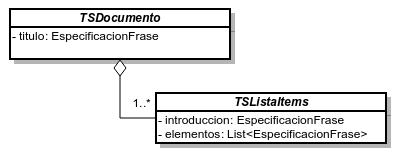
\includegraphics[scale=0.3]{img/text_spec.png}
	\caption{\emph{Text Specification}.}
  	\label{fig:text_spec}
\end{figure}

En la figura anterior podemos observar la estructura abstracta que tendrán nuestras \emph{text specification} y por ejemplo, sin meternos en detalle todavía sobre la estructura de las especificaciones de frase, en la figura \ref{fig:text_spec} podemos ver una especificación de frase para el ejemplo introducido anteriormente (pág. \pageref{fig:ej_corpus}).

\begin{figure}[H]
  	\centering
	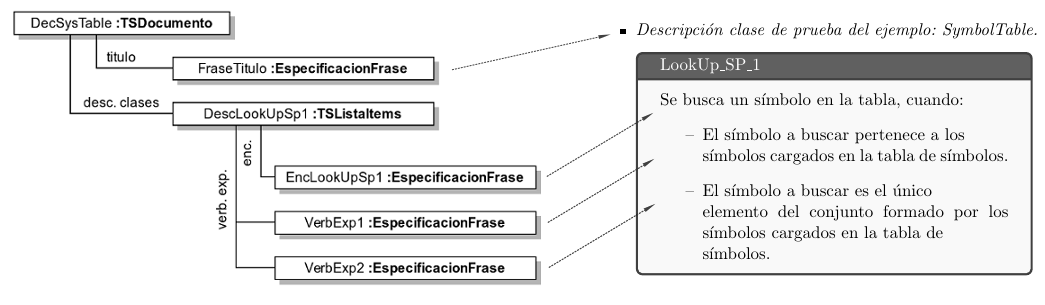
\includegraphics[scale=0.35]{img/ej_text_spec.png}
	\caption{Ejemplo \emph{Text Specification}.}
  	\label{fig:text_spec}
\end{figure}

Luego en la siguiente etapa, la de \emph{realización de estructura}, se deberán transformar estas estructuras en anotaciones para el sistema de presentación.

\subsection{Especificación de frase}

En la literatura sobre NLG Podemos encontrar muchas alternativas en lo que respecta a la especificación de frases. Todas estas varían en el nivel de abstracción que poseen las mismas. Las representaciones mas abstractas le darán mas flexibilidad a las etapas de \textit{document planning} y \textit{microplanning}, pero al mismo tiempo nos obligarán a tener un realizador de superficie mas sofisticado. Por otro lado, las especificaciones menos abstractas, requieren que el \textit{document planner} y el \textit{microplanner} realicen un mayor trabajo, pero también tendrán mas control sobre el texto a producir. Uno de los objetivos que tuvimos a la hora de idear una estructura para nuestra especificación de frases fue que ésta sea independiente de nuestro problema, pretendemos que hable en términos de la lengua (castellano en nuestro caso) que queremos generar y no en términos específicos de Z en nuestro caso. De esta forma podremos implementar un realizador de superficie que sea independiente de este problema y que pueda ser reutilizado. %TODO nota sobra la falta de un realizador en español al momento de desarrollar el trabajo


Es por esto que decidimos especificar las oraciones a generar mediante árboles sintácticos, donde los constituyentes de éstos serán los sintagmas\footnote{Grupo de palabras que ejercen una función sintáctica dentro de una oración} de la oración que deseamos generar. Esto le dará la posibilidad al realizador lingüístico de poder identificar la función de cada uno de los constituyentes de la oración. Por ejemplo, como detallamos en los requerimientos de la sección \ref{sec:microplanning_lexicalization}, el \emph{realizador de superficie} necesitará identificar el núcleo de un sintagma nominal (núcleo del sujeto) para poder producir frases en la que haya concordancia de número y persona entre el verbo y el sujeto de la oración. Como consecuencia del ejemplo anterior, nuestro sistema deberá tener la posibilidad de poder identificar el sujeto, predicado y verbo de una oración. A partir de un análisis del \emph{corpus} creemos que con los elementos presentes en la figura~\ref{fig:phase_spec} podremos modelar todas la frases que deberá producir nuestro sistema.

\begin{figure}[H]
  	\centering
	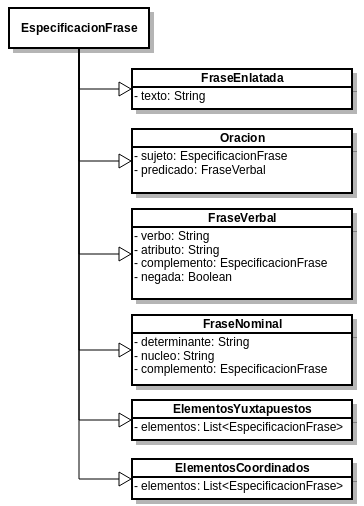
\includegraphics[scale=0.7]{img/phrase_spec.png}
	\caption{Phrase Specification.}
  	\label{fig:phase_spec}
\end{figure}

Como podemos notar no pretendemos modelar todo la lengua castellana con estos elementos sino solo un subconjunto que nos provea las herramientas necesarias permitirle al \emph{realizador de superficie} generar las frases definidas en el capítulo~\ref{sec:corpus_analisis}, ya que el desarrollo de un realizador lingüístico que tenga en cuenta todas las construcciones sintácticas de nuestra lengua escapa el alcance de nuestro trabajo. 

Es por esto que sólo modelaremos los sintagmas nominales (FraseNominal) y verbales (FraseVerbal) y nos veremos obligados a incluir otros elementos como \emph{ElementosYuxtapuestos} para salvaguardar la falta de algunos constituyentes sintácticos como sintagmas adjetivales, preposicionales, etc. 

A continuación describiremos brevemente cada uno de estos elementos, profundizando mas en detalle sobre la realización de los mismos en el capítulo~\ref{cap:linguistic_realization}.


\medskip
\begin{itemize}
\item{\emph{\textbf{FraseEnlatada}}: Representa texto que no necesita ningún tipo de procesamiento posterior a realizar durante la realización lingüística, será incluido en el texto tal cual fue establecido.}
\item{\emph{\textbf{Oración}}: Modela oraciones bimembres. El realizador lingüístico deberá procesarlas en base a una serie de reglas gramaticales para producir un texto sintáctica, morfológica y ortográficamente correcto para éstas.}
\item{\emph{\textbf{FraseVerbal}}: Representa un sintagma verbal que corresponderá al predicado de una \emph{Oración}.}
\item{\emph{\textbf{FraseNominal}}: Modela un sintagma nominal. Generalmente conformará el sujeto en una \emph{Oración}.}
\item{\emph{\textbf{ElementosCoordinados}}: Representa una serie de elementos que se deberán transformar en una conjunción de frases en la etapa de realización lingüística, por ejemplo: \emph{``frase1\textbf{,} frase2 \textbf{y} frase3''}}
\item{\emph{\textbf{ElementosYuxtapuestos}}: Representa una lista ordenada de elementos que deberán ser realizados y \emph{concatenados} en la oración final. Nos vimos obligados a introducir este tipo de elementos para salvaguardar la falta de algunos constituyentes sintácticos como sintagmas adjetivales, preposicionales, etc.}
\end{itemize}


%\section{Arquitectura}

\section{Lexicalización}
\label{sec:microplanning_lexicalization}

Como mencionamos anteriormente, el proceso de lexicalización será el encargado de elegir que palabras particulares y constructores sintácticos usar para comunicar la información contenida en el \textit{document plan}. En esta etapa deberemos producir una especificación de frase para cada mensaje contenido en el \textit{document plan}. En nuestro caso debemos hacerlo utilizando como especificación el conjunto de reglas definidas en el capítulo \ref{sec:corpus_reglas}, es decir, nuestro proceso de lexicalización tendrá que comportarse de la misma forma que la función \emph{verb} que estudiamos durante el análisis de requerimientos.

El módulo encargado de esta tarea deberá ser capaz de generar una \emph{especificación de frase} a partir de la expresión Z contenida en un mensaje del \emph{document plan}. Para esto, de acuerdo a los requerimientos introducidos en el capítulo \ref{cap:corpus}, primero deberemos verificar si la expresión en cuestión se encuentra designada, en este caso, tendrá que construir una especificación de frase en base a su designación. De lo contrario deberá intentar construirla recursivamente de acuerdo a las reglas antes mencionadas. En la figura~\ref{fig:algoritmo_lexicalizacion} podemos ver un bosquejo del comportamiento introducido en el análisis de requerimientos, trabajando esta vez con las \emph{phrase specification} definidas en la sección anterior. Incluimos sólo un bosquejo ya que ilustrar el comportamiento completo de esta tarea resulta extenso debido a la construcción y composición de sintagmas que debemos realizar para cada caso. 

\begin{algorithm}[H]
\caption{Bosquejo Lexicalización.}
\begin{algorithmic}
\Function {lexicalizacion}{$exp$}
\If{$esta\_designada(exp)$}
\State $ret\gets \text{designacion}(exp)$
\Else
\State $ret\gets \text{lexicalizacion'}(exp)$
\EndIf
\State \textbf{return} $ret$
\EndFunction
\Statex
\Function {lexicalizacion'}{$x = y$}
\State $fraseVerbal.verbo\gets \text{``es''}$
\State $fraseVerbal.atributo\gets \text{``igual''}$
\State $fraseEnlatada.texto\gets \text{``a''}$
\State $elemYuxtapuesto.elementos\gets \{fraseEnlatada, \text{lexicalizacion}(y)\}$
\State $fraseVerbal.complemento\gets elemYuxtapuesto$
\State $oracion.sujeto\gets \text{lexicalizacion}(x)$
\State $oracion.predicado\gets fraseVerbal$
\State \textbf{return} $oracion$
\EndFunction
\Statex
\ldots
\end{algorithmic}
\label{fig:algoritmo_lexicalizacion}
\end{algorithm}

La función \emph{designacion} deberá ser capaz de construir una especificación de frase a partir de una expresión designada. En la siguiente sección analizaremos este caso con mayor profundidad. Por otro lado, notemos que en el caso que la expresión a lexicalizar no se encuentre designada, se deberá analizar recursivamente la expresión para generar el texto adecuado según la especificación del capítulo \ref{sec:corpus_reglas}. 

Creemos que describir detalladamente nuestro algoritmo de lexicalización puede resultar muy engorroso para el lector debido a la cantidad de casos que debemos detallar (uno por cara regla de las antes mencionadas) y lo complejas que pueden resultar la creación y composición de especificaciones de frases. Es por esto que ilustraremos el resultado esperado de la tarea mediante un pequeño ejemplo. Intentaremos graficar nuestra tarea de verbalización para el primer \emph{mensaje} incluido en el \textit{document plan} de la figura \ref{fig:png_document_plan_ej}. Podemos observar en la figura \ref{fig:phase_spec_ej} este mensaje y la lexicalización del mismo. A continuación detallaremos los pasos realizados por nuestra tarea de lexicalización para obtener dicho resultado.

\begin{figure}
  	\centering
	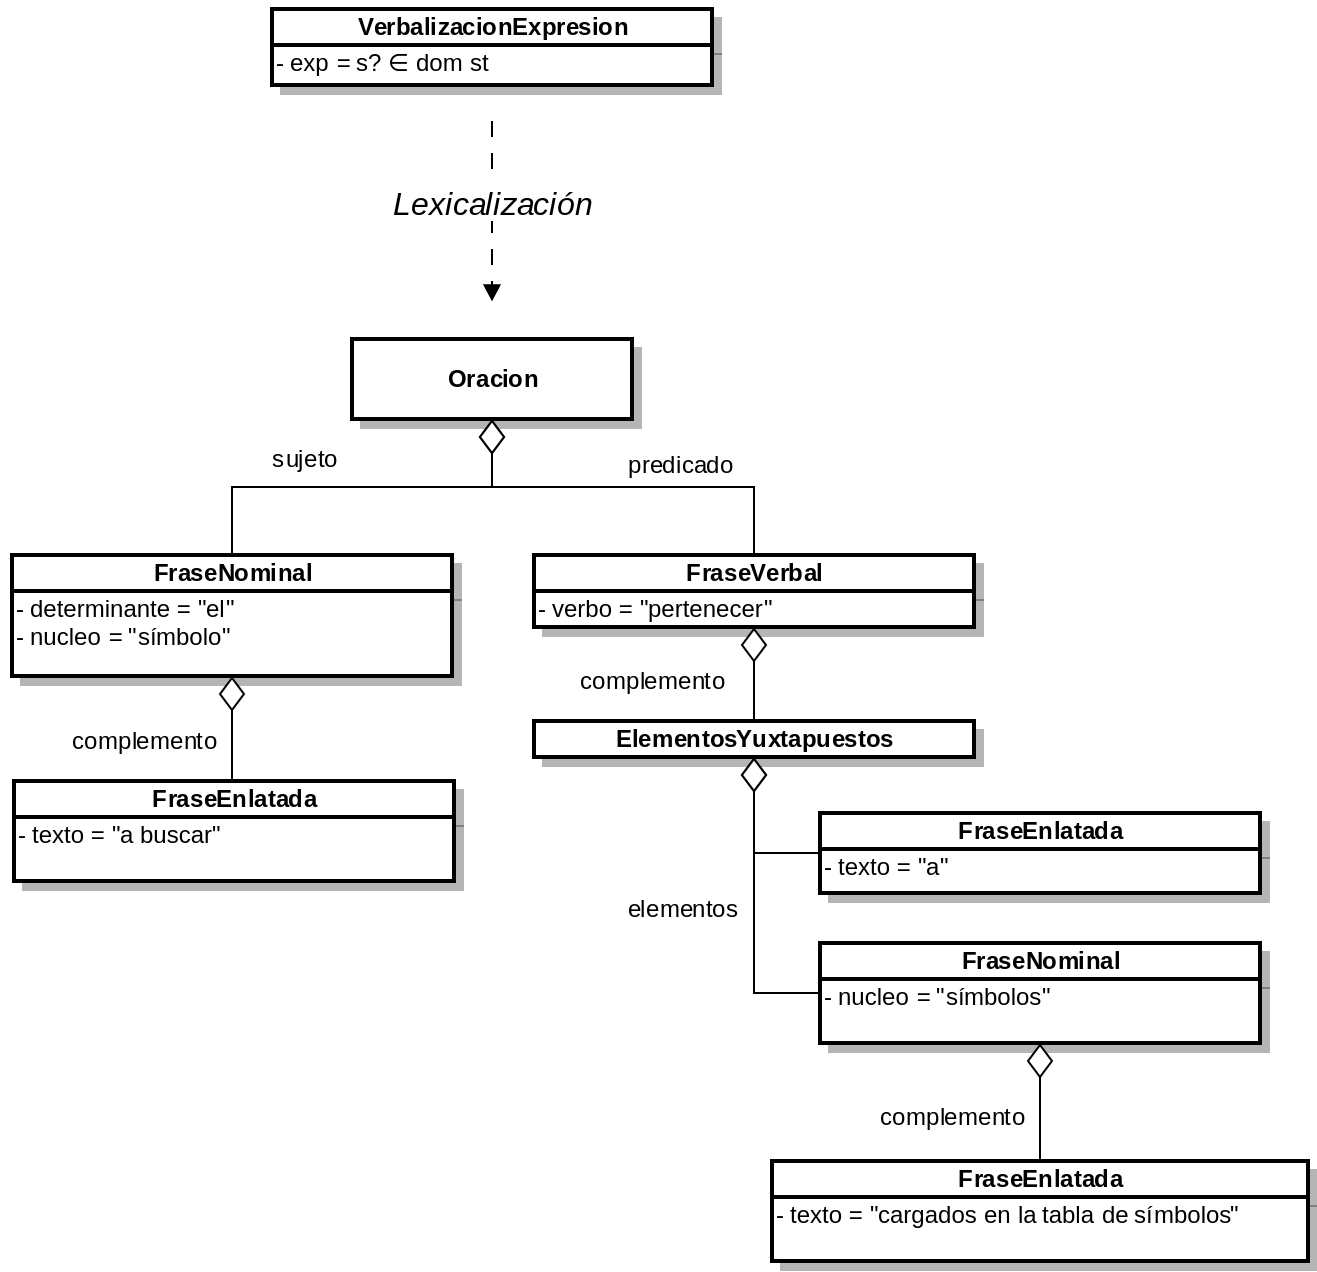
\includegraphics[scale=0.25]{img/phrase_spec_ej.png}
	\caption{Phrase Specification para $s? \protect\in \protect\dom st$.}
  	\label{fig:phase_spec_ej}
\end{figure}

Entonces, nuestra misión será lexicalizar la expresión:

\begin{center}
$s? \in \dom st$
\end{center}

\noindent
contando con las siguientes designaciones:

%TODO ver esto
\begin{align*} 
  &s? && \approx \text{el símbolo a buscar} \\
  &dom~x && \approx \text{símbolos cargados en la tabla de símbolos}
\end{align*}

En primer instancia, al no encontrarse designada $s? \in \dom st$ nuestro lexicalizador deberá construir una \emph{Oracion} para la frase:

\begin{center}
lexicalizacion $s?$ ++ ``pertenece a'' ++ lexicalizacion $\dom st$ 
\end{center}

Para esto deberá resolver recursivamente la lexicalizacion de $s?$ y de $\dom st$ para formar el \emph{sujeto} y \emph{predicado} necesarios para la oración. Luego deberá construir una \emph{FraseVerbal} utilizando tanto el \emph{verbo} como el \emph{complemento} a fin de obtener el texto ``pertenece a'' en el texto final.


Cabe aclarar que estableceremos el verbo en infinitivo siendo luego el realizador lingüístico el encargado de conjugar el mismo de acuerdo a algunas reglas gramaticales que veremos en el capítulo~\ref{cap:linguistic_realization}. Otra cuestión a mencionar es el uso del elemento \emph{ElementoYuxtapuestos} para salvaguardar la falta de un elemento que nos sirva para modelar un sintagma preposicional en este caso. Nuestro realizador lingüístico deberá procesar los elementos contenidos en cada \emph{ElementoYuxtapuestos} generando un texto resultado de la concatenación de la realización los mismos.


%TODO cambiar nombre
\section{Repositorio de designaciones}
\label{sec:verbalizacion_designaciones}
Como vimos en la sección anterior, nuestra tarea de lexicalización deberá hacer uso de las designaciones presentes en la especificación para la construir las especificaciones de clase. Para esto, nuestro sistema, cuando una expresión se encuentre designada, tendrá que procesar la misma, construyendo una especificación de frase que las caracterice. Esto será necesario ya que, como mencionamos previamente, en la etapa de \emph{realización de superficie} nuestro sistema necesitará conocer los distintos constituyentes sintácticos de las oraciones que les provee nuestra especificación de frase, en algunos casos también deberá, modificar levemente los textos incluidos en las designaciones.

Este modelado de frases a partir del texto de las designaciones deberá realizarse a medida que vamos procesando los distintos \emph{mensajes} del \textit{document plan} ya que será necesario conocer los argumentos utilizados en el caso de que debamos modelar una frase para una designación parametrizada.


%TODO designaciones parametrizadas = frase ya designada
%Los únicos predicados que uso del lado derecho son var \in set. Si eso te
% decir como verbalizar las designaciones parametrizadas, comentar lo complejo que sería debido que no sabemos cual es el orden, cual es el sujeto, cual el predicado, etc. asi que simplemente supondremos que es una frase enlatada

Un requerimiento que exigiremos al usuario para el uso de designaciones parametrizadas es que los posibles argumentos para estas expresiones que puedan aparecer en una clase de prueba también se encuentren designados. Por ejemplo, si tenemos la siguiente designacion en una especificación para un pequeño sistema de monitoreo de sensores:

\begin{align*} 
  &x \in dom smax && \approx \text{x es un identificador válido} 
\end{align*}

\medskip
\noindent
y tenemos la siguiente expresión en una de las clases de prueba que queremos describir:

\begin{center}
$s? \in \dom smax$
\end{center}

\noindent
sería deseable que la variable $s?$, en este caso, se encuentre designada. En el caso de este ejemplo lo está y la designacion para la misma es:

\begin{align*} 
  &s? && \approx \text{el identificador del sensor leído} 
\end{align*}

En este caso nuestro sistema simplemente remplazará el parametro con la designación correspondiente al argumento, quedando como resultado el siguiente texto:

\begin{center}
\emph{``el identificador del sensor leído es un identificador válido''}
\end{center}

Para poder construir una especificación de frase a partir del texto de una designación deberemos analizar síntacticamente la misma, para esto nuestro sistema deberá \textit{parsear} estas frases haciendo uso de un analizador morfológico. 

Para este trabajo requeriremos que el usuario escriba las designaciones como frases nominales. Es decir, esperamos que las designaciones posean la siguiente estructura:

\begin{figure}[H]
  \centering
   Sintagma Nominal = [Determinante] + Núcleo + [Complemento]
\end{figure}

Esto resulta algo bastante razonable y simplificará nuestro trabajo de \emph{parseo}. 
